\documentclass[aspectratio=169,10pt]{beamer}

\usepackage[T1]{fontenc}
\usepackage{lmodern}
\renewcommand{\familydefault}{\sfdefault}
\usepackage{amsmath,amssymb,amsthm}
\usepackage[mathscr]{eucal}
\usepackage{booktabs}
\usepackage{xcolor}

\usetheme{Madrid}
\definecolor{uorange}{HTML}{FF6F01}
\definecolor{uheadgold}{HTML}{FFCC03}
\usecolortheme[named=uorange]{structure}
\setbeamertemplate{navigation symbols}{}
\setbeamertemplate{itemize items}[circle]
\setbeamerfont{frametitle}{series=\bfseries}
% \setbeamertemplate{headline}{%
%   \noindent%
%   \colorbox{uheadgold}{\makebox[0.86\paperwidth]{\rule{0pt}{2.5mm}}}%
%   \colorbox{uorange}{\makebox[0.14\paperwidth]{\rule{0pt}{2.5mm}}}%
% }

\usepackage{tikz}
\usetikzlibrary{positioning,arrows.meta,calc,fit,backgrounds,shapes.geometric}

% ---- palette (used only to disambiguate the two chains in diagrams) ----
\definecolor{uink}{HTML}{15243B}
\definecolor{uacc}{HTML}{25607F}   % Unicity side
\definecolor{uext}{HTML}{9C5A12}   % external settlement chain
\definecolor{ugrn}{HTML}{2E6B4F}
\definecolor{ured}{HTML}{9B2D34}
\definecolor{ugry}{HTML}{5B6673}
\definecolor{ulit}{HTML}{EEF2F6}

% ---- yellowpaper notation (subset of common/definitions.tex) ----
\newcommand{\bytes}[1]{\mathbb{OCT}^{#1}}
\newcommand{\bool}{\mathbb{B}}
\newcommand{\predi}{\nu}
\newcommand{\auxd}{\mathsf{aux}}
\newcommand{\sthash}{{h_\mathsf{st}}}
\newcommand{\txhash}{{h_\mathsf{tx}}}
\newcommand{\zerohash}{\bot}
\newcommand{\Call}[2]{\textsc{#1}(#2)}
\newcommand{\Assets}{\textsc{Assets}}
\newcommand{\VerifyToken}{\textsc{VerifyToken}}
\newcommand{\LockFinal}{\textsc{LockFinal}}
\newcommand{\Prove}{\mathsf{Prove}}
\newcommand{\Verify}{\mathsf{Verify}}
\newcommand{\Root}{\mathsf{Root}}
\newcommand{\Insert}{\mathsf{Insert}}
\newcommand{\NonMember}{\mathsf{NonMember}}
\newcommand{\VerifyNonMember}{\mathsf{VerifyNonMember}}
\newcommand{\Hh}{H}
\newcommand{\cfg}{\mathcal{C}}
\newcommand{\hcfg}{h_\mathsf{cfg}}
\newcommand{\trust}{\mathcal{T}}
\newcommand{\accum}{A}
\newcommand{\nul}{\eta}
\newcommand{\bad}{\textcolor{ured}{\ding{55}}}

% ---- diagram styles ----
\tikzset{
  box/.style   ={rounded corners=1.5pt, draw=uink, line width=0.7pt, fill=ulit,
                 inner sep=5pt, align=center, font=\scriptsize},
  ubox/.style  ={box, draw=uacc, fill=uacc!8},
  ebox/.style  ={box, draw=uext, fill=uext!10},
  vbox/.style  ={box, draw=uink, fill=white, line width=1pt},
  note/.style  ={font=\scriptsize\itshape, text=ugry, align=center},
  flow/.style  ={-{Stealth[length=2.4mm]}, line width=0.9pt, draw=uink},
  uflow/.style ={flow, draw=uacc},
  eflow/.style ={flow, draw=uext},
}

% compact "definition strip"
\newcommand{\defn}[2]{\textbf{#1} --- #2}

\title[Unicity Asset Bridging]{Unicity Asset Bridging}
\subtitle{Bidirectional bridging between Unicity and an external settlement chain}
\author{Risto Laanoja}
\institute{Unicity Labs}
\date{\today}

\begin{document}

% ============================================================ Title
\begin{frame}
  \titlepage
%   \begin{center}\vspace{-1.2em}
%   \footnotesize Reference: Yellowpaper, \emph{Bridged Assets} and \emph{Asset Bridging}.
%   \end{center}
\end{frame}

% ============================================================ Summary
\begin{frame}{TL; DR summary}
\begin{itemize}\small
  \item Bidirectional bridging with \textbf{no trusted operator, committee,
        challenge window, or light client}.
  \item \textbf{Bridge-in}: a permissionless lock-backed mint each recipient
        verifies for itself; instant for the depositor.
  \item \textbf{Bridge-out}: a succinct validity proof compresses full token-history
        verification into one constant-cost on-chain check.
  \item On-chain replay state is a \textbf{single accumulator root}, rebuildable by
        anyone from public events.
  \item The prover is \textbf{disposable}: no authority, fully replaceable; a stall
        costs at most a fee.
  \item Chain-independent by construction: a new asset or chain is a new
        configuration and a new adapter, not new protocol.
  \item Trust reduces to one assumption: the settlement chain's own consensus.
\end{itemize}
\vskip1ex
\begin{center}\footnotesize
Full data structures, relation, algorithms:
Unicity Yellowpaper Appendix~\emph{Asset Bridging}.
\end{center}
\end{frame}

% ============================================================ Setting
\begin{frame}{Setting}
A fungible Unicity token may represent an asset held in custody on an
\emph{external chain} ($\chi$), like an account-based EVM/TVM chain. Bridging is
\textbf{bidirectional}:
\begin{itemize}
  \item \textbf{Bridge-in} (\emph{lock $\to$ mint}): lock the external asset in a
        settlement contract, the \emph{vault}; mint a Unicity token whose genesis
        \emph{backing reason} binds it to that lock.
  \item Now the token can be freely transacted on Unicity, can be split if it is fungible.
  \item \textbf{Bridge-out} / \emph{return} (\emph{burn $\to$ release}): burn the
        Unicity token; release the matching external asset from the vault.
\end{itemize}
% \vskip1ex
% {\footnotesize Throughout, $H = \mathsf{SHA\text{-}256}$ over deterministic CBOR
% encoding, and the vault's on-chain replay set is an authenticated (sparse Merkle)
% accumulator.}
\end{frame}

% ============================================================ Properties
\begin{frame}{Design properties}
\begin{columns}[T]
\begin{column}{0.52\textwidth}
\textbf{Trust}
\begin{itemize}\small
  \item No trusted operator, committee, challenge window.
  \item Return authorized only if verified by an immutable algorithm.
\end{itemize}
\vskip0.5ex
\textbf{User experience}
\begin{itemize}\small
  \item Bridge-in to one's own predicate is \emph{almost instant} (no finality wait for
        minting, finality on source blockchain needed for the first recipient).
  \item Bridge-out takes some time because of SNARK generation and batching.
  \item Minimal possible source blockchain fees.
  \item A stalled prover costs nothing; anyone can complete a return.
\end{itemize}
\end{column}
\begin{column}{0.48\textwidth}
\textbf{On-chain footprint}
\begin{itemize}\small
  \item Vault is one shared pool (one number)
  \item Returned asset replay state is \textbf{one accumulator root}.
  \item Constant-cost proof verification, independent of token history and batch
        size.
  \item Off-chain state is rebuildable from public source-blockchain events alone.
\end{itemize}
\vskip0.5ex
\textbf{Proving complexity}
\begin{itemize}\small
  \item History-dependent token verification is compressed into one succinct
        proof.
  \item Proving effort depends on batch size, and number of transactions per token. (sub-linear)
\end{itemize}
\end{column}
\end{columns}
\end{frame}

% ============================================================ System model
\begin{frame}{System model and trust base}
The vault is an external-chain contract that:
\begin{itemize}\small
  \item holds \emph{pooled} custody of one asset $a_\mathsf{A}$;
  \item has persistent storage;
  \item verifies a succinct proof for \emph{constant} cost;
  \item pins two immutable values:
  \begin{itemize}\footnotesize
    \item an allow-listed trust-base hash $h_\trust = H(\trust)$ --- \emph{which}
          Unicity Service instance is authoritative;
    \item a configuration hash $\hcfg$ committing the deployment.
  \end{itemize}
\end{itemize}
\vskip1ex
A deployment fixes a configuration
\[
  \cfg=(\chi,\;a_\mathsf{V},\;a_\mathsf{A},\;\mathsf{ty},\;\mathsf{aid},\;
        d_\mathsf{lock},\;d_\mathsf{nul},\;t_\mathsf{reason}),
\]
\[
  \hcfg=H(\mathsf{CFG\_DOMAIN},\;\chi,a_\mathsf{V},a_\mathsf{A},\mathsf{ty},
          \mathsf{aid},d_\mathsf{lock},d_\mathsf{nul},t_\mathsf{reason}).
\]
{\scriptsize
$\chi$ external chain id \quad
$a_\mathsf{V}$ vault (contract) address on $\chi$ \quad
$a_\mathsf{A}$ external asset (token contract) address \quad
$\mathsf{ty}$ bridged Unicity token type \\
$\mathsf{aid}$ asset identifier read from a token's payload \quad
$d_\mathsf{lock},d_\mathsf{nul}$ lock-digest / nullifier domain-separation tags \quad
$t_\mathsf{reason}$ CBOR tag of the return reason
}
\vskip0.5ex
{\footnotesize The vault derives $\hcfg$ \emph{and} its custody asset $a_\mathsf{A}$
from the same configuration value, so the asset the proof validates against and
the asset the vault pays out cannot diverge.}
\end{frame}

% ============================================================ Architecture
\begin{frame}{High-level architecture}
\begin{center}
\resizebox{\textwidth}{!}{%
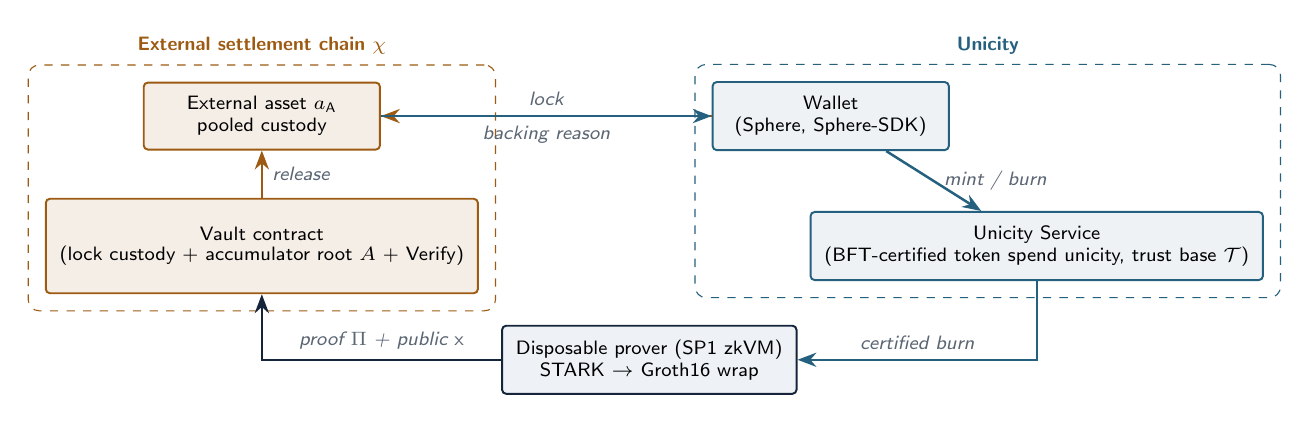
\begin{tikzpicture}[node distance=6mm]
  % external chain
  \node[ebox, minimum width=30mm, minimum height=12mm] (vault) {Vault contract\\[-1pt]\scriptsize(lock custody + accumulator root $\accum$ + $\Verify$)};
  \node[ebox, above=6mm of vault, minimum width=30mm] (asset) {External asset $a_\mathsf{A}$\\\scriptsize pooled custody};
  \begin{scope}[on background layer]
    \node[draw=uext, dashed, rounded corners, fit=(vault)(asset), inner sep=6pt,
          label={[uext,font=\scriptsize\bfseries]above:External settlement chain $\chi$}] {};
  \end{scope}
  % unicity side
  \node[ubox, right=42mm of asset, minimum width=30mm] (wallet) {Wallet\\\scriptsize(Sphere, Sphere-SDK)};
  \node[ubox, right=42mm of vault, minimum width=30mm] (us) {Unicity Service\\\scriptsize(BFT-certified token spend unicity, trust base $\trust$)};
  \begin{scope}[on background layer]
    \node[draw=uacc, dashed, rounded corners, fit=(wallet)(us), inner sep=6pt,
          label={[uacc,font=\scriptsize\bfseries]above:Unicity}] {};
  \end{scope}
  % prover
  \node[box, below=10mm of $(vault)!0.5!(us)$, minimum width=34mm] (prover) {Disposable prover (SP1 zkVM)\\\scriptsize STARK $\to$ Groth16 wrap};

  % flows
  \draw[eflow] (wallet.west) -- node[note,above]{lock} (asset.east);
  \draw[uflow] (asset.east) -- node[note,below]{backing reason} (wallet.west);
  \draw[uflow] (wallet) -- node[note,right]{mint / burn} (us);
  \draw[uflow] (us.south) |- node[note,near end,above]{certified burn} (prover.east);
  \draw[flow] (prover.west) -| node[note,near start,above]{proof $\Pi$ + public $\mathsf{x}$} (vault.south);
  \draw[eflow] (vault.north) -- node[note,right]{release} (asset.south);
\end{tikzpicture}}
\end{center}
% \vskip-0.5ex
% {\footnotesize Three independent components (vault, wallet/SDK, prover) on three
% stacks. The single hard rule: all three produce and consume \emph{byte-identical}
% encodings and hashes ($\hcfg$, nullifier, reason). ($\mathsf{x}$, the public
% statement the proof attests to, is spelled out in full later.)}
\end{frame}

% ============================================================ Asymmetry
\begin{frame}{In vs out}
The two directions are \emph{not} symmetric, because the two chains have different
finality semantics and different verification costs.
\vskip1ex
\begin{columns}[T]
\begin{column}{0.5\textwidth}
\textbf{Bridge-in} \hfill {\scriptsize external $\to$ Unicity}
\begin{itemize}\small
  \item External locks have \emph{probabilistic} finality.
  \item A recipient must confirm the lock is final on $\chi$.
  \item Realized as a \emph{mint-reason verifier} each recipient re-runs
        (reading external state).
  \item Cost of verification is small and client-side; the wait is intrinsic to the
        external chain.
\end{itemize}
\end{column}
\begin{column}{0.5\textwidth}
\textbf{Bridge-out} \hfill {\scriptsize Unicity $\to$ external}
\begin{itemize}\small
  \item A Unicity burn is BFT-final the instant it is certified; offline-verifiable
        by $\VerifyToken{}$.
  \item The vault has high gas fees: re-running $\VerifyToken{}$ on-chain
        is prohibitively expensive, grows with number of txs accumulated.
  \item Realized as a \emph{succinct validity proof} that compresses the
        history-dependent check off-chain into one constant-cost verification.
\end{itemize}
\end{column}
\end{columns}
\vskip1.5ex
\begin{center}\footnotesize
Bridge-in has a finality \emph{wait} but trivial verification;
bridge-out has instant finality but needs a compact \emph{proof}.
\end{center}
\end{frame}

% ============================================================ Bridge-in mechanics
\begin{frame}{Bridge-in: lock, record, mint}
\begin{columns}[T]
\begin{column}{0.54\textwidth}
The locker fixes the recipient predicate $\predi'_0$ and a salt, determining
\[
  \mathsf{id}=H(\mathsf{salt},\alpha),\quad h_\mathsf{rcpt}=H(\mathsf{CBOR}(\predi'_0)).
\]
The vault escrows the asset, assigns a monotone lock nonce $n$, and emits a
\emph{lock event}
\[
  L_\mathsf{lock}=(n,\;a_\mathsf{src},\;v,\;\mathsf{id},\;h_\mathsf{rcpt}).
\]
{\scriptsize $\alpha$: Unicity network id \quad $a_\mathsf{src}$: depositor \quad
$v$: locked amount.}
It stores \emph{only} the \emph{lock digest} of the record
$\mathcal{K}=(a_\mathsf{A},\mathsf{ty},\mathsf{aid},v,\mathsf{id},h_\mathsf{rcpt})$:
$d=H(\mathsf{LOCK\_DOMAIN},\chi,a_\mathsf{V},n,\mathcal{K})$,
$\mathsf{lockDigest}[n]\gets d$
--- {\scriptsize $d$ is the \emph{only} return-relevant state the vault keeps.}
\end{column}
\begin{column}{0.46\textwidth}
\begin{center}
\resizebox{\columnwidth}{!}{%
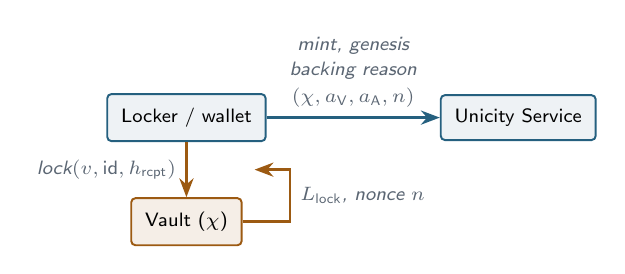
\begin{tikzpicture}[node distance=5mm]
  \node[ubox] (L) {Locker / wallet};
  \node[ebox, below=7mm of L] (V) {Vault ($\chi$)};
  \node[ubox, right=22mm of L] (U) {Unicity Service};
  \draw[eflow] (L) -- node[note,left]{lock$(v,\mathsf{id},h_\mathsf{rcpt})$} (V);
  \draw[eflow] (V.east) -- ++(0.6,0) |- node[note,near start,right]{$L_\mathsf{lock}$, nonce $n$} ($(L.east)!0.5!(V.east)$);
  \draw[uflow] (L) -- node[note,above]{\shortstack{mint, genesis\\backing reason\\$(\chi,a_\mathsf{V},a_\mathsf{A},n)$}} (U);
\end{tikzpicture}}
\end{center}
\vskip1ex
{\footnotesize Minting is \emph{permissionless}: the minter key is a public constant
derived from $\mathsf{id}$. Authority comes entirely from the backing reason.}
\end{column}
\end{columns}
\end{frame}

% ============================================================ Backing verification
\begin{frame}{Bridge-in: backing verification}
Every recipient runs the token-type mint-reason check against the pinned $\cfg$
and an external-finality oracle $\LockFinal{\chi,a_\mathsf{V},n}$, on
$D_\mathsf{mint}$, the genesis's mint-reason data:
\vskip0.5ex
\begin{block}{\textsc{VerifyBackingReason}$(D_\mathsf{mint},\trust,\cfg)$ (essentials)}
\footnotesize
\begin{enumerate}
  \item decode $(\mathsf{ver},\chi',a'_\mathsf{V},a'_\mathsf{A},n)$; ensure
        $\mathsf{ver}{=}1$ and $(\chi',a'_\mathsf{V},a'_\mathsf{A})$ equal the
        pinned trust anchors;
  \item $(\mathsf{ok},a''_\mathsf{A},v,\mathsf{id}_L,h_\mathsf{rcpt})\gets
        \LockFinal{\chi',a'_\mathsf{V},n}$; ensure $\mathsf{ok}{=}1$,
        $a''_\mathsf{A}{=}a'_\mathsf{A}$;
  \item ensure $\mathsf{id}_L=H(\mathsf{salt},\alpha)$ \hfill \emph{(lock funds this exact token)}
  \item ensure $h_\mathsf{rcpt}=H(\mathsf{CBOR}(\predi'))$ \hfill \emph{(lock binds this recipient)}
  \item ensure locked amount $v=$ genesis value for $\mathsf{aid}$ \hfill \emph{(no inflation)}
\end{enumerate}
\end{block}
\vskip0.5ex
{\footnotesize The reason body carries \emph{only} the lock locator and trust
anchors. Every security-relevant value --- identifier, recipient, amount --- is read
from the certified genesis and the lock event and checked against each other,
never trusted from the reason.
\par\smallskip
$\LockFinal{}$ is the one step Unicity cannot internalize: a live $\chi$ query with
$K$ confirmations (a fixed confirmation-depth threshold), \emph{or} a carried
inclusion proof against a pinned $\chi$ anchor. This is the bridge's only
external-chain assumption.}
\end{frame}

% ============================================================ Bridge-in security
\begin{frame}{Bridge-in: security}
An accepted bridged genesis implies a final lock on $\chi$ committing to the same
identifier, recipient, and amount. Enumerated guarantees:
\vskip1ex
\begin{itemize}\small
  \item \defn{No mint without a lock}{genesis accepted only against a matching
        \emph{final} lock.}
  \item \defn{No double mint}{one genesis per $\mathsf{id}$; the lock commits to
        $\mathsf{id}$, so one lock funds exactly one token.}
  \item \defn{No theft}{$h_\mathsf{rcpt}$ binds ownership to the named predicate;
        only the intended recipient can spend.}
  \item \defn{No value inflation}{declared genesis value must equal the locked
        amount.}
  \item \defn{No rogue contract}{chain, vault, and asset must equal the pinned
        $\cfg$.}
  \item \defn{No reorged lock}{the lock must be final on $\chi$.}
\end{itemize}
\vskip1ex
{\footnotesize The wait is enforced by each verifier for itself, not attached to
the token as a global condition. The locker minting to a predicate it already
controls needs \emph{no} wait --- it witnessed its own deposit; a wallet may show
such a token to its owner immediately. Only the first party that did \emph{not}
witness the lock must run $\LockFinal{}$.}
\end{frame}

% ============================================================ Bridge-out setting
\begin{frame}{Bridge-out: setting and return authorization}
\begin{columns}[T]
\begin{column}{0.56\textwidth}
A Unicity burn is final the instant it is BFT-certified and verifiable offline by
$\VerifyToken{}$ against the trust base $\trust$ alone.
\vskip1ex
To return, the holder forms a \emph{return reason} $\mathcal{R}$ and burns the token with
\[
  \auxd'=b_\mathcal{R},\qquad \predi'=\predi_\mathsf{burn}(H(CBOR(\mathcal{R}))),
\]
{\footnotesize where $\auxd'$ is the burn transaction's auxiliary-data field and
$\predi'$ its next (here: burn) predicate.}
$\mathcal{R}$ is therefore part of the \emph{certified} burned token, not a
separate witness the prover supplies.
\end{column}
\begin{column}{0.44\textwidth}
\footnotesize
\textbf{Return reason} $\mathcal{R}$ (public):
\begin{tabular}{@{}ll@{}}
\toprule
$0$ & version $=1$\\
$1$--$5$ & $\chi,a_\mathsf{V},a_\mathsf{A},\mathsf{ty},\mathsf{aid}$ (pinned)\\
$6$ & $a_\mathsf{r}$ external recipient\\
$7$ & $v$ gross $=$ burned value for $\mathsf{aid}$\\
$8$--$9$ & $a_\mathsf{f},v_\mathsf{f}$ optional relayer fee\\
$10$ & $t_d$ deadline (gates the fee only)\\
\bottomrule
\end{tabular}
\vskip1ex
Every field is public by nature --- the external release is a public event. The
\emph{private} part of a return is the token's transfer history, which never
leaves the witness.
\end{column}
\end{columns}
\end{frame}

% ============================================================ Nullifier
\begin{frame}{Bridge-out: the nullifier}
Replay prevention uses a \emph{nullifier accumulator} --- an authenticated set of
already-released burns, whose root $\accum$ the vault stores on-chain.
\vskip1ex
The nullifier is derived from the certified burn leaf. For the final certified
transfer (burn transaction) $T_\mathsf{b}$, spending state $(\predi_{n-1},\sthash_{n-1})$
--- predicate and state hash of the token just before the burn --- with data
field $D$ and data hash $\txhash_\mathsf{b}=H(T_\mathsf{b}.D)$:
\[
  \mathsf{sid}_\mathsf{b}=H(\predi_{n-1},\sthash_{n-1}),\qquad
  \mathsf{btid}_\mathsf{b}=H(\mathsf{BURN\_DOMAIN},\mathsf{sid}_\mathsf{b},\txhash_\mathsf{b}),
\]
\[
  \boxed{\;\nul=H(\mathsf{NUL\_DOMAIN},\;\hcfg,\;\mathsf{btid}_\mathsf{b})\;}
\]
\vskip1ex
{\footnotesize $\mathsf{sid}_\mathsf{b}$ is recorded \emph{at most once} by the
Unicity Service (the same mechanism that prevents double-spending), so $\nul$ is
globally unique. The certified $\txhash_\mathsf{b}$ binds it to the exact return
reason; $\hcfg$ separates deployments so the same burn never collides across
independent bridges. A release proves $\nul \notin \accum$ and inserts it; the
vault advances $\accum$. On-chain replay state stays \textbf{constant} --- one
root.}
\end{frame}

% ============================================================ Bridge-out flow
\begin{frame}{Bridge-out: flow}
\begin{center}
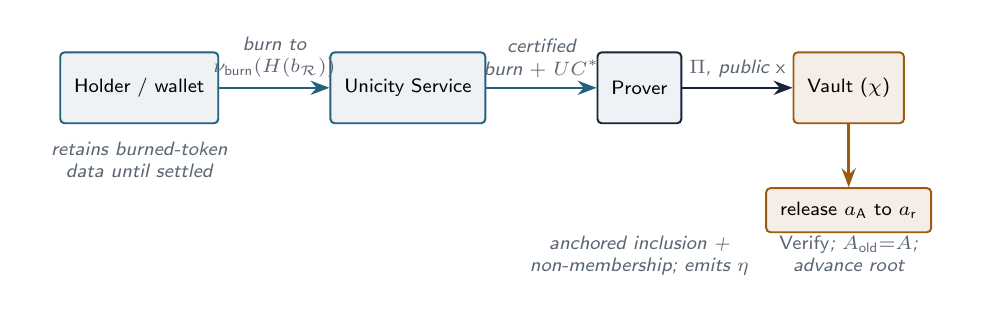
\begin{tikzpicture}[node distance=10mm]
  \node[ubox, minimum height=9mm] (h) {Holder / wallet};
  \node[ubox, right=14mm of h, minimum height=9mm] (u) {Unicity Service};
  \node[box,  right=14mm of u, minimum height=9mm] (p) {Prover};
  \node[ebox, right=14mm of p, minimum height=9mm] (v) {Vault ($\chi$)};

  \draw[uflow] (h) -- node[note,above]{burn to\\$\predi_\mathsf{burn}(H(b_\mathcal{R}))$} (u);
  \draw[uflow] (u) -- node[note,above]{certified\\burn $+$ $UC^*$} (p);
  \draw[flow]  (p) -- node[note,above]{$\Pi$, public $\mathsf{x}$} (v);
  \draw[eflow] (v.south) -- ++(0,-8mm) node[ebox, below, minimum width=20mm] (r) {release $a_\mathsf{A}$ to $a_\mathsf{r}$};

  \node[note, below=1mm of h, text width=26mm] {retains burned-token data until settled};
  \node[note, below=13mm of p, text width=30mm] {anchored inclusion + non-membership; emits $\nul$};
  \node[note, below=13mm of v, text width=26mm] {$\Verify$; $\accum_\mathsf{old}{=}\accum$; advance root};
\end{tikzpicture}
\end{center}
\vskip1ex
{\footnotesize $UC^*$ is a recent Unicity certificate anchoring the burn's
inclusion proof (defined next). The prover cannot alter recipient or amount
(fixed in the certified $\mathcal{R}$) nor fabricate a release; it can only
stall. Any party holding the burned token can reproduce the proof and submit it.}
\end{frame}

% ============================================================ Validity statement
\begin{frame}{The validity statement}
The public statement committed by the proof and checked by the vault is
\[
  \mathsf{x}=(\hcfg,\;h_\trust,\;\accum_\mathsf{old},\;\accum_\mathsf{new},\;
             \mathsf{rr},\;\mathsf{lr},\;B,\;V),
\]
with $\accum_\mathsf{old}/\accum_\mathsf{new}$ the accumulator transition, $B$ the
batch size, $V$ the total gross amount, and $\mathsf{rr},\mathsf{lr}$ vector
commitments to the release leaves and lock references.
\vskip1ex
For a batch of $B$ burns the proof attests the conjunction:
\begin{itemize}\small
  \item \defn{Anchor}{one recent certificate $UC^*$ certifies SMT root $h^*$ under
        $\trust$, and $H(\trust)=h_\trust$.}
  \item \defn{Finality}{each burned token verifies by $\VerifyToken{}$, every leaf
        included under the shared $h^*$; the final state is a burn whose reason is
        $\mathcal{R}$.}
  \item \defn{Value \& backing}{each burned amount equals the certified value for
        $\mathsf{aid}$, tracing --- through split value-conservation --- to a genesis
        whose backing references a recorded lock.}
  \item \defn{Destination}{each $\mathcal{R}$ matches $\cfg$ and yields a public
        release leaf $(\nul,a_\mathsf{r},v,a_\mathsf{f},v_\mathsf{f},t_d)$.}
  \item \defn{Replay}{each $\nul$ absent from $\accum_\mathsf{old}$; inserting them
        yields $\accum_\mathsf{new}$.}
\end{itemize}
\end{frame}

% ============================================================ Relation
\begin{frame}{The batch proving relation $\mathfrak{R}(\mathsf{x},\mathsf{w})$}
Witness $\mathsf{w}$: the config $\cfg$, trust base $\trust$, anchor $UC^*$, and per
burn $i$ the source token $\mathcal{L}_i$, its anchored inclusion proofs, the
backing lock record, and a non-membership witness $w_i$.
\vskip0.5ex
{\footnotesize
$H_\mathsf{cfg}(\cfg)=\mathsf{x}.\hcfg$;\quad $H(\trust)=\mathsf{x}.h_\trust$;\quad
verify $UC^*$ once, $h^*\gets UC^*.IR.h$; \quad $\accum\gets\mathsf{x}.\accum_\mathsf{old}$.
\par\smallskip
\textbf{for each} $i=1\ldots B$:}
\begin{enumerate}\footnotesize
  \item $\VerifyToken{\mathcal{L}_i,\trust}$ in \emph{anchored} mode against $h^*$;
        recompute $\mathsf{sid}_{\mathsf{b},i},\txhash_{\mathsf{b},i}$ from the final
        certified burn.
  \item decode $\mathcal{R}_i$ from the burn aux; ensure fields $1$--$5$ equal $\cfg$.
  \item value $v_i$ from the genesis for $\mathsf{aid}$; ensure
        $\mathcal{R}_i.v=v_i$ and $\mathcal{R}_i.v_\mathsf{f}\le v_i$.
  \item backing: recompute $d_i=H(\mathsf{LOCK\_DOMAIN},\chi,a_\mathsf{V},n_i,\mathcal{K}_i)$;
        ensure $\mathcal{K}_i$ binds this $\mathsf{id}$, recipient, $\mathsf{aid}$, $v_i$.
  \item replay: $\nul_i$ from the burn; ensure $\VerifyNonMember(\accum,\nul_i,w_i)$;
        $\accum\gets\Insert(\accum,\nul_i,w_i)$.
\end{enumerate}
{\footnotesize \textbf{final:} $\accum=\mathsf{x}.\accum_\mathsf{new}$, $\sum v_i=\mathsf{x}.V$,
$\mathsf{Commit}(\text{leaves})=\mathsf{x}.\mathsf{rr}$,
$\mathsf{Commit}(\text{lockrefs})=\mathsf{x}.\mathsf{lr}$.}
\end{frame}

% ============================================================ Anchored inclusion
\begin{frame}{Anchored inclusion: one certificate per batch}
Because the Unicity SMT is \textbf{add-only}, every state a token ever occupied
remains provable under any later root. So one recent certificate anchors entire
token histories.
\vskip1ex
\begin{itemize}\small
  \item Fix an anchor certificate $UC^*$ with root $h^*=UC^*.IR.h$.
  \item For each certified transaction leaf $L=(\mathsf{sid},\txhash)$, carry an SMT
        inclusion certificate $C^\mathsf{inc}$ of $L$ against $h^*$.
  \item The relation verifies $UC^*$ \emph{once} via $\mathsf{VerifyUnicityCert}$,
        then each $L$ by a hash-path check $\mathsf{VerifyMember}(h^*,L,C^\mathsf{inc})$.
\end{itemize}
\vskip1ex
This replaces $m$ BFT-certificate verifications (one per transaction leaf $L$
across all burned tokens' histories) by \textbf{one} certificate plus $m$
hash-path checks --- the dominant saving inside the circuit.
\vskip1ex
{\footnotesize Anchored inclusion omits the original request-validation time, so
the relation is defined only for \emph{time-independent} predicates
(signature/burn/split). Time-dependent predicates (timelocks/HTLCs) require
carrying authenticated validation time --- future scope.}
\end{frame}

% ============================================================ Trustless
\begin{frame}{Trustless setup}
No party --- including the deployer --- can move funds except by presenting a
mathematically valid proof against an \emph{immutable} relation.
\vskip1ex
\begin{itemize}\small
  \item \defn{Immutable $\mathsf{vk}$}{the verification key is fixed at deployment;
        the relation cannot be silently swapped. Changing it requires a \emph{new}
        vault (\S upgrades).}
  \item \defn{Prover holds no authority}{recipient and amount are fixed inside the
        certified $\mathcal{R}$; the prover can only stall, never steal or forge.}
  \item \defn{Each recipient is its own verifier}{bridge-in acceptance is a check
        every recipient re-runs; no bridge party attests to anything.}
  \item \defn{No committee, no challenge window}{the vault releases funds
        \emph{only} against a valid succinct proof --- there is nothing to
        optimistically trust and later dispute.}
  \item \defn{Authenticity by soundness}{$\mathfrak{R}$ embeds $\VerifyToken{}$
        against the pinned $\trust$; a forged, malformed, or non-final burn is
        unrepresentable under proof-system knowledge-soundness.}
\end{itemize}
\vskip1ex
\begin{center}\footnotesize
The \emph{only} external assumption is the settlement chain's own consensus
(bridge-in finality) --- nothing else is trusted.
\end{center}
\end{frame}

% ============================================================ Disposable prover
\begin{frame}{The disposable prover}
The prover is a pure function of \emph{public} inputs plus the holder-retained
burned-token data. It has no keys, no custody, no privileged state --- so it is
fully replaceable.
\vskip1ex
\begin{columns}[T]
\begin{column}{0.54\textwidth}
\textbf{Liveness argument.} From the on-chain root and the public
$\mathsf{Released}$ event stream, \emph{any} party can:
\begin{enumerate}\small
  \item rebuild the off-chain accumulator to $\accum$;
  \item refetch anchored inclusion proofs from the Unicity Service;
  \item reproduce the proof and submit it.
\end{enumerate}
\vskip0.5ex
The only residual requirement is availability of the burned-token data, which the
holder retains until settlement.
\end{column}
\begin{column}{0.46\textwidth}
\footnotesize
\textbf{Consequences}
\begin{itemize}
  \item A stalled or absent relayer costs at most the fee $v_\mathsf{f}$: after the
        deadline the recipient receives the full amount, and anyone --- including
        the recipient --- may submit.
  \item The prover can be a self-hosted, single-machine, sequential process. No
        Docker, no GPU, no proving network required for correctness.
  \item A defective prover cannot damage the vault; at worst it produces no proof.
\end{itemize}
\end{column}
\end{columns}
\end{frame}

% ============================================================ Contracts
\begin{frame}{The on-chain contract set}
\begin{columns}[T]
\begin{column}{0.5\textwidth}
\textbf{Vault} (one per deployment) --- persistent state:
\begin{itemize}\footnotesize
  \item $\mathsf{vk}$, $\hcfg$, custody asset $a_\mathsf{A}$;
  \item allow-list of trust-base hashes (rotatable under timelock);
  \item bridge-in map $\mathsf{lockDigest}[\cdot]$;
  \item accumulator root $\accum$ (init $\accum_\emptyset$).
\end{itemize}
\vskip0.5ex
\textbf{Entry points}
\begin{itemize}\footnotesize
  \item $\mathsf{lock}(v,\mathsf{id},h_\mathsf{rcpt})$ --- escrow, assign $n$, store
        $d$, emit $L_\mathsf{lock}$.
  \item $\textsc{FulfilBatch}(\mathsf{x},\Pi,\langle\ell_i\rangle,\langle(n_j,d_j)\rangle)$
        --- $\ell_i$ a release leaf $(\nul,a_\mathsf{r},v,a_\mathsf{f},v_\mathsf{f},t_d)$,
        $(n_j,d_j)$ the referenced lock nonces/digests.
  \item $\mathsf{setTrustBaseAllowed}$ (timelocked, governance).
\end{itemize}
\vskip0.5ex
\textbf{$\mathsf{SP1Verifier}$} --- one global bn254 Groth16 verifier, shared by all
vaults.
\end{column}
\begin{column}{0.5\textwidth}
\textbf{$\textsc{FulfilBatch}$} (settlement):
\begin{enumerate}\footnotesize
  \item $\Verify(\mathsf{vk},\mathsf{x},\Pi)=1$;
  \item $\mathsf{x}.\hcfg=\hcfg$, $\mathsf{x}.h_\trust\in$ allow-list;
  \item $\mathsf{x}.\accum_\mathsf{old}=\accum$ \hfill\emph{(the entire replay guard)}
  \item commitments $\mathsf{rr},\mathsf{lr}$ re-checked; each
        $\mathsf{lockDigest}[n_j]=d_j$;
  \item $\accum\gets\mathsf{x}.\accum_\mathsf{new}$ \hfill\emph{(one root update)}
  \item pay each leaf; fee only if $\mathsf{now}\le t_d$ and $a_\mathsf{f}\ne\bot$;
  \item emit $\mathsf{Released}(\nul,\dots)$, $\mathsf{BatchFulfilled}(\dots)$.
\end{enumerate}
\vskip0.5ex
{\footnotesize No external query, no light client: the proof self-certifies its
anchor under the allow-listed $\trust$; backing is confirmed against locally
recorded digests. The vault tracks \emph{no} Unicity roots.}
\end{column}
\end{columns}
\end{frame}

% ============================================================ Minimal on-chain data
\begin{frame}{On-chain data is minimal}
The vault keeps only what is needed to be safe; \emph{nothing} that grows with
Unicity history.
\vskip1ex
\begin{center}\small
\begin{tabular}{@{}lll@{}}
\toprule
State & Size & Grows with \\
\midrule
$\mathsf{vk}$, $\hcfg$, $a_\mathsf{A}$ & constant & --- (immutable) \\
Trust-base allow-list & tiny & validator-set epochs \\
Accumulator root $\accum$ & \textbf{one hash} & --- (constant) \\
$\mathsf{lockDigest}[n]$ & one hash / deposit & bridge-in deposits \\
\bottomrule
\end{tabular}
\end{center}
\vskip1ex
\begin{itemize}\small
  \item Replay prevention for the entire return history is a \textbf{single root}.
  \item No per-transition certificates, no Unicity roots, no token histories are
        ever stored on-chain.
  \item The split (decision): keccak256/ABI for vault-recomputed commitments
        ($\hcfg$, $d$, $\mathsf{rr}$, $\mathsf{lr}$); SHA-256/CBOR for
        Unicity-internal values ($\nul$, accumulator, $h_\trust$) that the vault
        never recomputes.
\end{itemize}
\end{frame}

% ============================================================ Accumulator reconstruction
\begin{frame}{Nullifier tree: reconstruct from on-chain data alone}
The accumulator is a depth-256 sparse Merkle tree keyed by $\nul$, leaf value
$\mathtt{0x01}$. It is \textbf{deterministically rebuildable by anybody} from
public events, based on data availability guarantee of the source blockchain.
\vskip0.5ex
\begin{center}
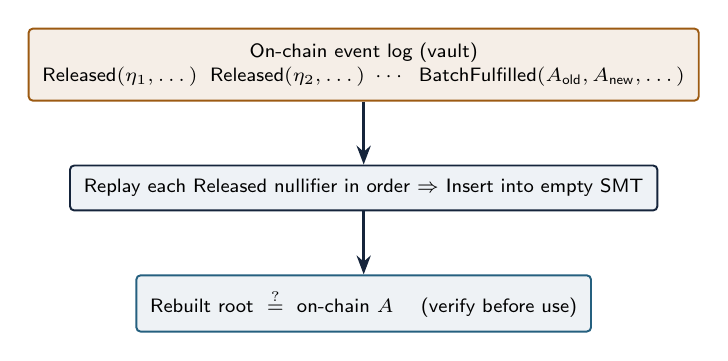
\begin{tikzpicture}[node distance=6mm, every node/.style={font=\scriptsize}]
  \node[ebox, minimum width=52mm] (log) {On-chain event log (vault)\\[1pt]
     $\mathsf{Released}(\nul_1,\dots)\;\;\mathsf{Released}(\nul_2,\dots)\;\cdots\;\;\mathsf{BatchFulfilled}(\accum_\mathsf{old},\accum_\mathsf{new},\dots)$};
  \node[box, below=8mm of log, minimum width=52mm] (rb) {Replay each $\mathsf{Released}$ nullifier in order $\Rightarrow$ $\Insert$ into empty SMT};
  \node[ubox, below=8mm of rb, minimum width=52mm] (chk) {Rebuilt root $\;\stackrel{?}{=}\;$ on-chain $\accum$ \quad(verify before use)};
  \draw[flow] (log) -- (rb);
  \draw[flow] (rb) -- (chk);
\end{tikzpicture}
\end{center}
\vskip0.5ex
\begin{itemize}\footnotesize
  \item $\mathsf{Released}$ emits each nullifier; $\mathsf{BatchFulfilled}$ emits each
        root transition --- so the off-chain accumulator is rebuildable from public
        data alone and \emph{verified against the on-chain $\accum$} before use.
  \item The service additionally re-verifies the rebuilt root equals the vault's
        on-chain root (SYNCED gate) before building a new batch.
\end{itemize}
\end{frame}

% ============================================================ Settlement properties
\begin{frame}{Settlement properties}
\begin{itemize}\small
  \item \defn{No external query, no light client}{the proof self-certifies its
        anchor; backing checked against local digests; the vault tracks no Unicity
        roots.}
  \item \defn{Fee optionality never strands funds}{$t_d$ and $a_\mathsf{f}$ gate the
        fee \emph{only}. After the deadline, or when $a_\mathsf{f}=\bot$, the
        recipient gets the full amount; anyone may submit.}
  \item \defn{Batch atomicity}{all $B$ transfers settle together; a reverting
        recipient reverts the batch, but $\accum$ is unchanged and no nullifier is
        consumed --- a liveness, not a safety, concern. A deployment expecting
        blockable recipients may credit withdrawable balances instead.}
  \item \defn{Reconstructability}{$\mathsf{Released}$ + $\mathsf{BatchFulfilled}$
        make the accumulator rebuildable from public data.}
\end{itemize}
\vskip1ex
{\footnotesize \textbf{Implementation note.} On EVM/TVM chains a low-level asset
transfer may not receive the caller's full remaining gas/energy after an expensive
proof verification in the same transaction; the vault budgets an explicit
sufficient fee per transfer rather than relying on default forwarding.}
\end{frame}

% ============================================================ Economics
\begin{frame}{Economics of batching}
The public statement and settlement procedure are identical for every batch size
$B$; only the prover changes. The $\approx$constant proof verification is shared
across the whole batch, so per-return cost falls as $1/B$.
\vskip0.5ex
\begin{columns}[T]
\begin{column}{0.5\textwidth}
\footnotesize
\[
  \textsc{FulfilBatch}(B)\approx 267\text{,}779 + 19\text{,}347\cdot B \;\text{(energy)}
\]
\begin{tabular}{@{}rrr@{}}
\toprule
$B$ & per-return energy & per-return \$$^\ast$ \\
\midrule
$1$   & $287\text{,}126$ & $\sim\!9.0$ \\
$10$  & $46\text{,}125$  & $\sim\!1.5$ \\
$100$ & $22\text{,}025$  & $\sim\!0.7$ \\
$\infty$ & $19\text{,}347$ & $\sim\!0.6$ \\
\bottomrule
\end{tabular}
\vskip0.5ex
{\scriptsize $^\ast$Tron mainnet, measured Nile energy, 210 sun/energy, \$0.15/TRX (burn model).}
\end{column}
\begin{column}{0.5\textwidth}
\footnotesize
\textbf{Cost structure}
\begin{itemize}
  \item Proof verify ($\sim\!218$k energy) is \emph{per batch} $\Rightarrow$
        amortizes $1/B$.
  \item Only the $\sim\!19$k/return transfer + leaf checks are truly per-return.
  \item Off-chain proving is one Groth16 proof per batch --- chain-agnostic;
        amortizes $1/B$ too.
  \item Staking energy (Tron) turns the recurring fee into refundable capital
        $\Rightarrow$ marginal on-chain cost $\to 0$.
\end{itemize}
\vskip0.5ex
The relayer fronts energy and is reimbursed via $v_\mathsf{f}$; the vault enforces
$v_\mathsf{f}\le v$ and pays the fee only before $t_d$.
\end{column}
\end{columns}
\end{frame}

% ============================================================ New asset / chain
\begin{frame}{Integrating the next asset and the next chain}
The relation $\mathfrak{R}$ and the vault are \textbf{chain-independent}; a new
deployment is a new configuration, not new protocol.
\vskip1ex
\begin{itemize}\small
  \item \defn{New asset, same chain}{fix a fresh $\cfg$ (new $a_\mathsf{A}$,
        $\mathsf{ty}$, $\mathsf{aid}$), deploy a vault with the resulting $\hcfg$,
        publish $\hcfg$ + allowed $h_\trust$. The circuit is unchanged.}
  \item \defn{New chain}{select chain-specific parameters --- address width, the
        $\LockFinal{}$ realization ($K$ confirmations or a pinned anchor), the
        vector-commitment primitive --- and redeploy. The settlement chain is
        abstracted as ``contract with storage + verifier''.}
  \item \defn{Wallet/SDK side}{a neutral \texttt{@unicitylabs/bridge-core} defines
        \texttt{BridgeSourceAdapter} / \texttt{ChainWallet} / \texttt{ChainClient};
        a chain is added as a \emph{new adapter} producing opaque \texttt{Step[]}
        (e.g.\ ERC-20 \texttt{approve+lock} vs.\ single-signature EIP-3009). The
        wallet's state machine is identical.}
\end{itemize}
\vskip1ex
{\footnotesize The manifest is a discriminated union keyed on chain family with a
CAIP-2 chain reference; adding a family is additive, never a fork. The generic
justification payload carries the full $\hcfg$ --- identifying vault \emph{and}
complete trusted configuration in one field.}
\end{frame}

% ============================================================ Software components
\begin{frame}{Implementation: software components}
\begin{columns}[T]
\begin{column}{0.52\textwidth}
\textbf{Monorepo \texttt{github.com/unicitylabs/unicity-bridge}}
\begin{itemize}\scriptsize
  \item \texttt{protocol/} --- the normative byte contract
        (\texttt{interop.md}) + conformance vectors every stack must reproduce.
  \item \texttt{contracts/tron/} --- vault \& lock TVM contracts
        (\texttt{UnicityBridgeVault}, \texttt{UnicityLock}, SP1-verifier binding),
        Hardhat tests.
  \item \texttt{packages/bridge-core} --- chain-neutral TS interfaces
        (\texttt{BridgeSourceAdapter}/\texttt{ChainWallet}/\texttt{ChainClient}).
  \item \texttt{packages/bridge-plugin-tron-usdt} --- first chain plugin: Tron
        USDT verifier, wallet adapter, CLI/demo.
  \item \texttt{prover/} --- Rust/SP1 return-prover workspace: \texttt{core}
        (no\_std byte contract), \texttt{guest} (SP1 circuit), \texttt{host},
        \texttt{sdk-ext} (bridge-only extensions over the token SDK),
        \texttt{service} (return service).
  \item \texttt{deployments/} --- frozen deployment metadata.
\end{itemize}
\end{column}
\begin{column}{0.48\textwidth}
\textbf{Wallet side}
\begin{itemize}\scriptsize
  \item \texttt{sphere} @ \texttt{feat/unicity-bridge} --- the wallet UI/UX
        (display, bridge-in/out flows).
  \item \texttt{sphere-sdk} @ \texttt{feat/unicity-bridge} --- fa\c{c}ade +
        manifest wiring (previous/next frame).
\end{itemize}
\vskip1ex
\textbf{The Rust SDK}\\
\texttt{\scriptsize{github.com/unicitynetwork/state-transition-sdk-rust}}
\begin{itemize}\scriptsize
  \item \texttt{no\_std}-first and zkVM-ready \emph{by design} --- it is what
        the SP1 guest links against to re-verify full token history
        \emph{inside the circuit}.
  \item Wallets/services that don't prove keep using the existing
        \texttt{state-transition-sdk-js}; the Rust SDK was developed specifically to
        make in-circuit verification possible.
\end{itemize}
\end{column}
\end{columns}
\end{frame}

% ============================================================ Sphere integration
\begin{frame}{Sphere / SDK integration}
\begin{columns}[T]
\begin{column}{0.5\textwidth}
\textbf{Boundary (hard rule).} Sphere holds no bridge
logic: all derivations and chain specifics are provided by the plugin; Sphere imports a
\emph{fa\c{c}ade} + a \emph{manifest} and renders UI.
\vskip0.5ex
\footnotesize
\texttt{buildBridgeInPlan} $\to$ \{tokenId, recipientCommitment, approveTx, lockTx\}\\
\texttt{buildBridgeBackPlan} $\to$ \{burnTransfer, preview, witnessRequest\}\\
\texttt{previewReturn}, \texttt{decodeBridgeBackReason} (read-only UI).
\vskip0.5ex
The SDK exposes \texttt{bridges: BridgeManifest[]}; plugins are built via the
fa\c{c}ade and their justification verifiers forwarded into the token engine ---
no core engine change.
\end{column}
\begin{column}{0.5\textwidth}
\textbf{User-facing flows}
\begin{itemize}\footnotesize
  \item \textbf{Display}: bridged balances carry a ``bridged (USDT $\cdot$ Tron)''
        badge; unknown/failed re-verify $\to$ ``unverified'', excluded from
        spendable; ``confirming ($N$ blocks)'' during finality.
  \item \textbf{Bridge in}: \texttt{approve} (one-time) $\to$ \texttt{lock} $\to$
        mint at \texttt{confirmations:0} (self-trust) $\Rightarrow$ token spendable
        immediately; pending-lock recovery resumes an interrupted mint.
  \item \textbf{Bridge out}: pick a returnable balance, dest + amount; sign the
        Unicity burn; persist the burned blob (recovery-critical); poll the return
        service \emph{and} watch \texttt{Released\{$\nul$\}}; self-settle after the
        deadline.
\end{itemize}
\end{column}
\end{columns}
\vskip0.5ex
{\footnotesize A ``returnability'' flag (time-independent-predicate lineage) gates
``Bridge out''. Cross-stack conformance vectors keep Solidity, TypeScript, and
Rust byte-identical.}
\end{frame}


% ============================================================ Upgrades
% \begin{frame}{Relation and configuration upgrades}
% $\mathsf{vk}$ and $\hcfg$ are fixed at deployment and \emph{cannot} be changed in
% place. This rigidity is the direct consequence of what makes the vault
% trustworthy.
% \vskip1ex
% \begin{itemize}\small
%   \item $\hcfg$ is self-referential through $a_\mathsf{V}$: a new vault address
%         necessarily yields a new $\hcfg$. Relocating custody and changing the
%         relation are mechanically the same event.
%   \item A relation upgrade (fix or extend $\mathfrak{R}$):
%   \begin{enumerate}\footnotesize
%     \item deploy a new vault with the new $\mathsf{vk}$/$\hcfg$, empty accumulator,
%           empty lock-digest map, no allow-listed trust base;
%     \item publish the new configuration; stop bridge-in against the old vault;
%     \item return outstanding value under the \emph{old} relation --- the new vault
%           has no record of old locks.
%   \end{enumerate}
% \end{itemize}
% \vskip1ex
% {\footnotesize \textbf{Migration discipline}: a redeploy is \emph{not} ``old stuff
% becomes stale''. Assets stay locked in the old vault and existing tokens retain
% claims against it; keep the old manifest, verifier, and return service operational
% until old-vault liabilities reach zero.}
% \end{frame}

% ============================================================ Security summary
\begin{frame}{Security properties (summary)}
\begin{itemize}\small
  \item \defn{Solvency}{every bridged token is backed by an equal lock; split
        verification bounds children by their parent; the backing check ties each
        burn to a recorded lock digest. Hence $\sum(\text{released})\le
        \sum(\text{locked})$ --- custody cannot be over-drawn.}
  \item \defn{Replay-freeness}{nullifiers are globally unique; each release proves
        non-membership and inserts; the vault requires $\accum_\mathsf{old}=\accum$.
        A resubmitted proof fails (root advanced); a fresh proof cannot show
        non-membership of an inserted nullifier.}
  \item \defn{Authenticity \& finality}{$\mathfrak{R}$ embeds $\VerifyToken{}$
        against the pinned $\trust$; by knowledge-soundness an accepting proof
        implies a genuine, BFT-final burn whose reason is exactly $\mathcal{R}$.}
  \item \defn{Liveness, data availability}{the prover holds no authority and is replaceable; any party
        rebuilds the accumulator from public data (the source blockchain) and reproduces a proof. Residual
        requirement: availability of the burned-token data, retained by the holder.}
\end{itemize}
\end{frame}



\end{document}
